% DNS defined in the intro!
\subsection{Incompressible DNS FFT Kernel}
\label{sec:dns}

In many fluid dynamics applications, turbulence plays a
dominant role. Unfortunately, turbulence is notoriously complex and
difficult to model.  One reliable
tool for analyzing turbulence is direct
numerical simulation (DNS)\cite{jimenez:2007}, where Navier--Stokes numerical solutions
are fully resolved
in both time and space. 
%%%Although DNS is too
%%%computationally expensive for engineering calculations, high quality
%%%DNS is an excellent tool for investigation of turbulent flow physics.  

% However, the extremely high resolution requirements of DNS
% require excellent system performance. 
% Communication costs arise from large volume of data all-to-all exchanges
% between nodes needed to perform transposes. Direct matrix solves for the
% wall-normal component of velocity rely on processor clockspeeds. Due to
% the large problem sizes, the code is also memory intensive, and depends
% on memory bandwidth and cache size available; finally, writing large
% amounts of data for postprocessing makes I/O performance critical.

%The simulation code seeks the solution of the
%time-dependent three-dimensional incompressible Navier--Stokes
%equations. Periodic boundary conditions are imposed in the streamwise
%and span-wise direction, while in the wall normal direction, no slip
%conditions are imposed at the walls. A partially implicit third order
%Runge-Kutta/Crank--Nicholson scheme is used for time discretization. 
%In

In the DNS application used
by PECOS to simulate channel flow, a Fourier spectral
representation is used in the streamwise and spanwise directions,
while a high order compact finite difference is used in the
wall-normal direction\cite{KMM:87,Lele:92}.
%%%% picture of channel
%%%\begin{figure}[h]
%%%\begin{center}
%%% 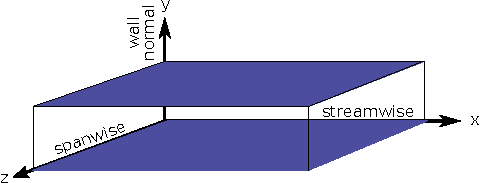
\includegraphics[height=.39\linewidth]{geometry}
%%% \caption{The Channel Geometry.}
%%%\end{center}
%%%\end{figure}
The Fourier method allows a natural decoupling between different modes
in transformed space such that multiple tasks can operate on their own data
independently. Our method uses a 2D decomposition which divides an $N_x
\times N_y \times N_z$ domain into M pencils. Fourier transforms in 3D
are performed one direction at a time, and transposes 
re-partition the domain into pencils aligned in appropriate
directions,
as depicted in Figure~\ref{fig:pencil2}. This
paper focuses on single-node performance.  Thus,
for the kernel discussed below, the final pencil depicted (x,z,y) is
the portion of the domain considered for FFT analysis on MIC.

% picture of pencils
\begin{figure}[htb]
 \begin{center}
  \includegraphics[width=0.35\textwidth]{PencilTransposeSchematic}
  \caption{The two dimensional data decomposition. The localized FFT
    on the pencil shown on the far right is ported to the KNF MIC platform.}
    \label{fig:pencil2}
 \end{center}
\end{figure}

Algorithmically, the final inverse Fourier transform, physical space
calculations, and the first Fourier transform into wavespace are
performed completely on-node and do not require MPI subroutine calls. 
Previously the inverse Fourier transform, realspace calculations,
and forward transform were performed separately. This section of code
was re-factored to perform all three steps on each line of the pencil
individually. These changes improved cache coherency and optimized the
algorithm for multithreading, the performance and scaling of which is
the basis for this section. 

The resulting FFT kernel was run with a pencil size of $\{N_x,N_z, N_y\} =$ 
(8192,1280,1), with $N_x$ corresponding to the direction being
Fourier transformed. This was iterated over six pencils to emulate
the real DNS code, which requires operating on three velocity components
($u$,$v$,$w$) as well as the non-linear terms ($uu$,$uv$,$ww$) required
to resolve the velocity at the subsequent timestep. The size of the
pencil was chosen to correspond to a realistic pencil size for a a
single compute node during a large scale DNS simulation, where the
global mesh size would be (8192,12288,1024). 

The kernel application code is written entirely in Fortran-90, and
uses OpenMP for multithreading to perform multiple 2D
FFTs simultaneously.
%and requires a series of
%two-dimensional FFTs to complete the analysis.  

We compare results from FFTW 3.3 to the FFTW interface in MKL.  Runs
were made at various thread counts on both the host Westmere and KNF
MIC platforms and the results were verified analytically. Timings were
averaged over two successive runs, and results comparing FFTW to MKL
performance are shown in
Figure~\ref{fig:mkl-vs-fftw}. Figure~\ref{fig:mkl-vs-fftw}(a) compares
the speedup factor obtained using MKL on Westmere with observed
performance increases ranging from $\sim$20-40\%.
Figure~\ref{fig:mkl-vs-fftw}(b) shows results on MIC, where the
performance increases with MKL are more dramatic, suggesting that the
FFT implementation within MKL enables more vectorization than the FFTW
counterpart. This performance difference also impacts scalability on
MIC, as shown in Figure~\ref{fig:dns_scaling}.  In this case, the
speedup factor is based on a baseline case with four threads.  The MKL
implementation scales much better than the FFTW version. With 120
threads, an overall scaling efficiency of 72\% was achieved using MKL,
whereas only 35\% was achieved with FFTW.

% completed on both the
%FFTW for Fourier transforms. The code is
%essentially a series of DO loops that iterate over the z and y
%directions. 

To quantify the impact of various runtime affinity settings available
on MIC, Figure~\ref{fig:dns_affinity} presents the real-to-complex
(Fourier transform into frequency space) performance gains for several
thread affinity options: scatter, compact or
explicit. Results in Figure~\ref{fig:dns_affinity} are
all compared against the default case: no KMP\_AFFINITY setting.
For both MKL and FFTW
linkage, the {\em scatter} setting provided the best overall
performance across a wide thread-count range.  Note that this
setting was seen to have a significant impact on observed runtimes.

%% From the provided Intel
%% documentation:
%% \begin{itemize}

%%  \item \textbf{Scatter}: ``Specifying scatter distributes the threads as
%%        evenly as possible across the entire system. scatter is the
%%        opposite of compact; so the leaves of the node are most
%%        significant when sorting through the machine topology map.'' 

%%  \item \textbf{Compact}: ``Specifying compact assigns the OpenMP thread
%%        $\langle n \rangle + 1$ to a free thread context as close as
%%        possible to the thread context where the $\langle n \rangle$
%%        OpenMP thread was placed.''

%%  \item \textbf{Explicit}:``Specifying explicit assigns OpenMP threads to
%%        a list of OS proc IDs that have been explicitly specified by
%%        using the proclist$=$ modifier, which is required for this affinity
%%        type. ''
%% \end{itemize}



% need to add discussion of affinity results here
% http://software.intel.com/sites/products/documentation/studio/composer/en-us/2011/compiler_c/optaps/common/optaps_openmp_thread_affinity.htm#Explicitly_Specifying_OS_Proc_IDS__GOMP_CPU_AFFINITY 

\begin{figure}[htp]
\begin{center}
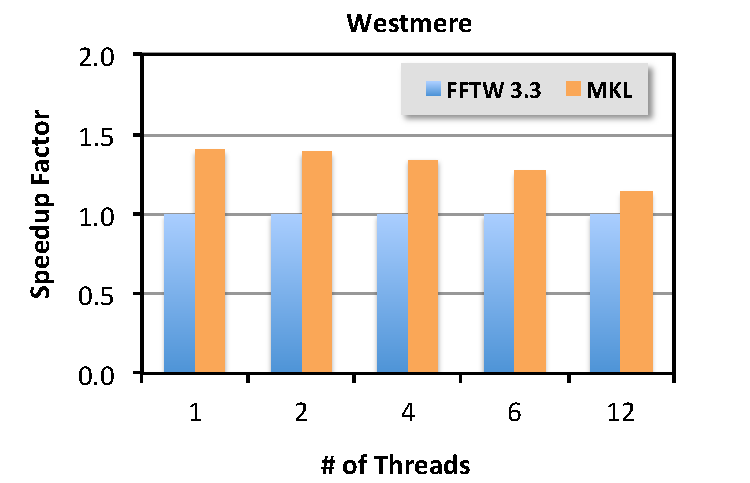
\includegraphics[width=0.95\linewidth]{dns_westmere_fftw_vs_mkl.pdf}
(a)
\includegraphics[width=0.95\linewidth]{dns_mic_fftw_vs_mkl.pdf} 
(b)
\end{center}
\vspace*{-.5cm}
\caption{Relative comparison between threaded FFT kernel
  used in DNS applications on (a) dual-socket Westmere server and (b)
  KNF MIC co-processor.}
\label{fig:mkl-vs-fftw}
\end{figure}

\begin{figure}[h]
\begin{center}
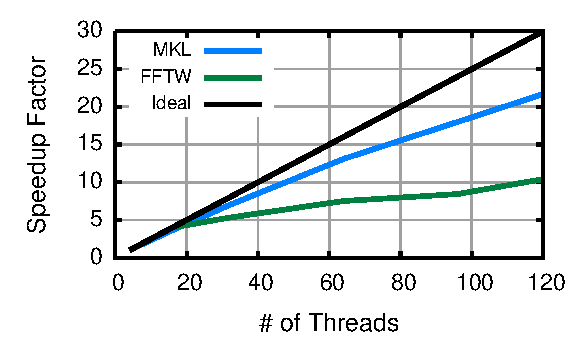
\includegraphics[width=0.9\linewidth]{dns-fftw-scaling.pdf}
\end{center}
\vspace*{-.5cm}
\caption{Scaling of DNS FFT kernel on KNF MIC accelerator ({KMP\_AFFINITY=scatter}).}
\label{fig:dns_scaling}
\end{figure}

\begin{figure}[htp]
\begin{center}
\includegraphics[width=1.0\linewidth]{dns_affinity_mkl.pdf}
(a)
\includegraphics[width=1.0\linewidth]{dns_affinity_fftw3.pdf}
(b)
\end{center}
\vspace*{-.5cm}
\caption{Influence of runtime affinity setting on MIC.
  Relative performance change is based
  on comparison to runs with no affinity setting provided. A
  positive performance change indicates faster runtimes.  Results are
  presented for FFTs performed with the (a) MKL and (b) FFTW3
  libraries.}
\label{fig:dns_affinity}
\end{figure}




%

%\begin{figure}[htp]
%\begin{center}
%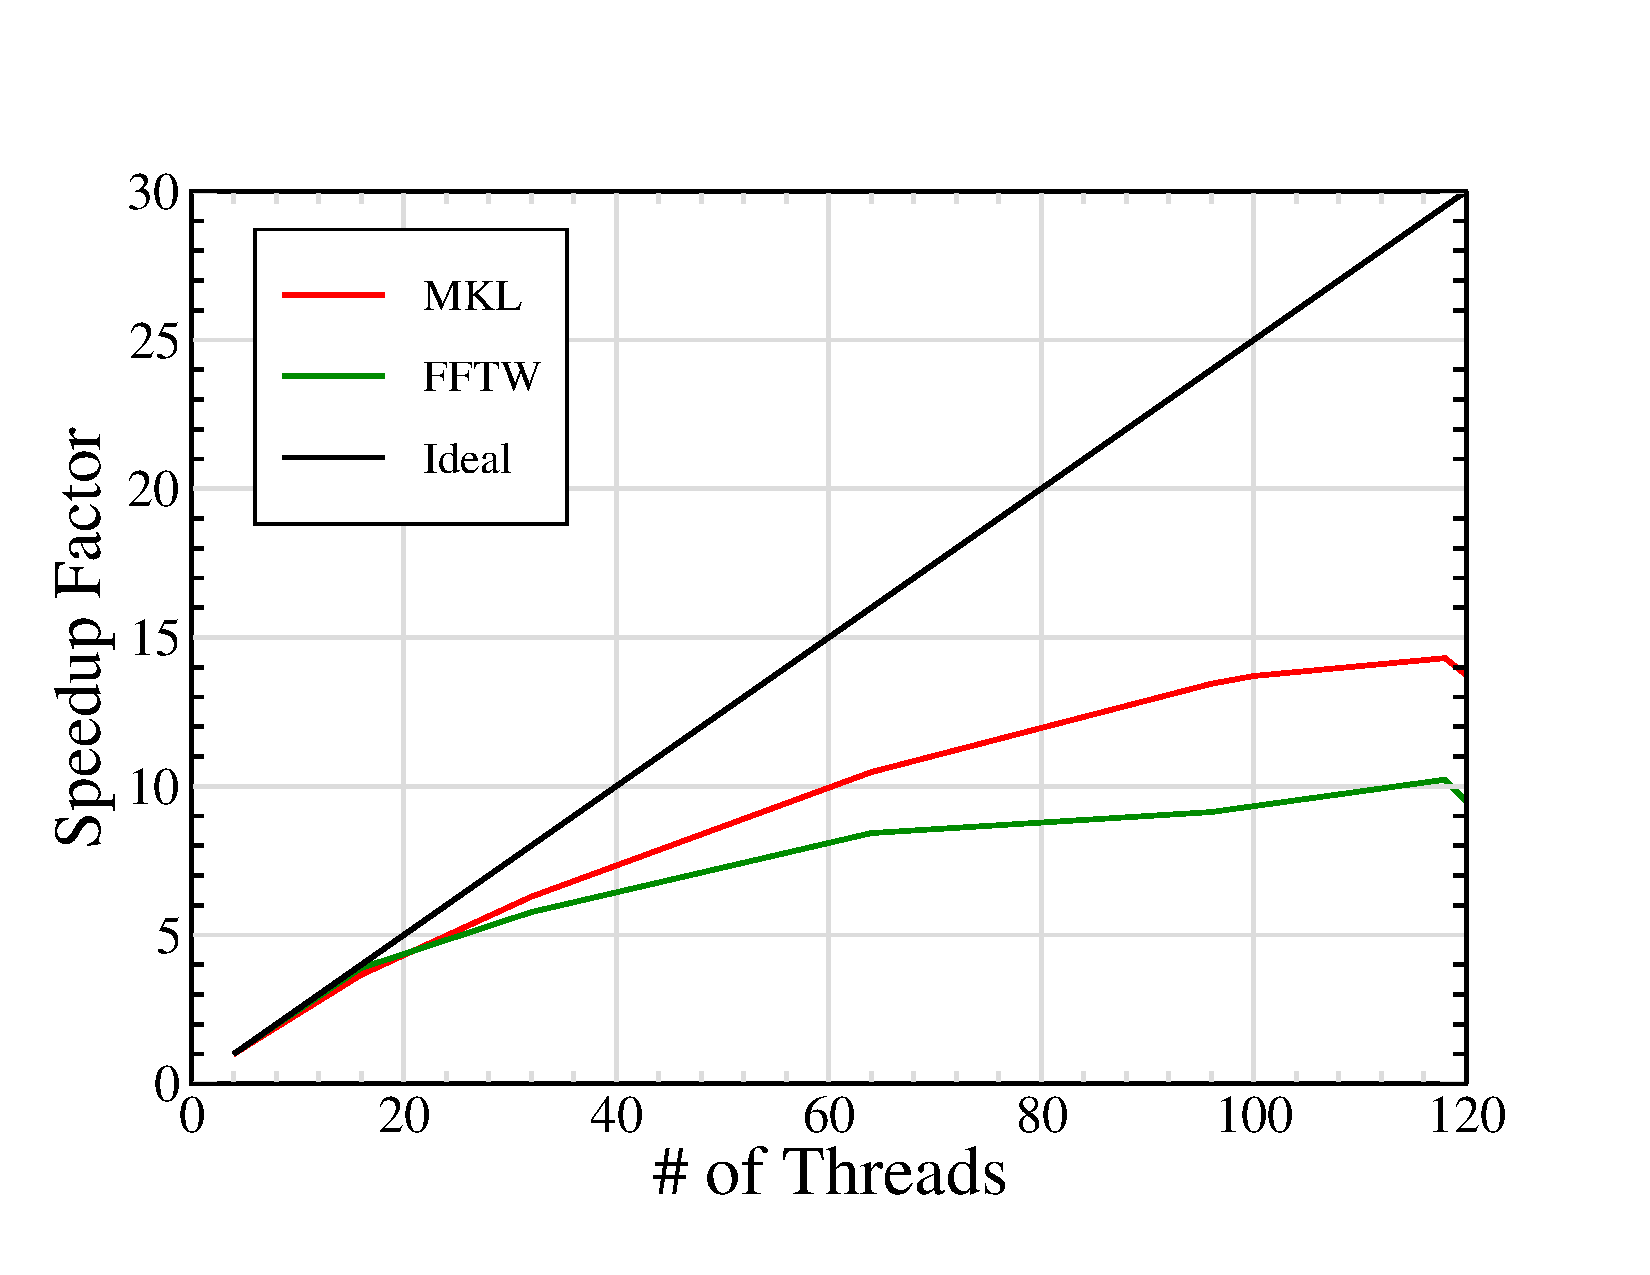
\includegraphics[width=1.0\linewidth]{dns_full_kernel.pdf}
%\end{center}
%\vspace*{-.5cm}
%\caption{Scaling of the Complex-to-Real FFT, Nonlinear computations and
% Complex-to-Real FFT DNS kernel on KNF MIC accelerator.}
%\label{fig:dns_scaling}
%\end{figure}
%
